\documentclass{report}
\usepackage[a4paper]{geometry}

\usepackage{graphicx} \graphicspath{ {./figures/} }
\usepackage{booktabs}
\usepackage{amsthm, amsmath, amssymb, amsfonts}
\usepackage{float, subcaption}
\usepackage{datetime}
%\usepackage{titlespec}

\usepackage{hyperref}
\hypersetup{pdftex}
\usepackage{hypcap}

\usepackage{fontspec}
\usepackage{polyglossia}
\setmainlanguage[Script=Cyrillic]{serbian}
\setotherlanguage{english}
\setmainfont{Times New Roman}

\usepackage{fancyhdr}
\fancyhead[L]{Примена теорије група}
\fancyhead[R]{Даниел Силађи, IV-9}
%\fancyfoot[C]{\thepage}

\theoremstyle{plain}
\newtheorem{thm}{Теорема}
\newtheorem*{lem}{Лема}
\newtheorem*{cor}{Последица}
\theoremstyle{definition}
\newtheorem*{defn}{Дефиниција}

\newcommand{\HRule}{\rule{\linewidth}{0.5mm}}


\begin{document}
\pagestyle{fancy}

\begin{titlepage}
\begin{center}
\Large\textbf{Гимназија ,,Јован Јовановић Змај''}\\
\Large Нови Сад\\[8.7cm]
\LARGE\bfseries Матурски рад из Анализе са алгебром\\[3mm]
\LARGE\bfseries ПРИМЕНА ТЕОРИЈЕ ГРУПА\\
\end{center}
\vfill
\begin{minipage}{0.5\textwidth}
\begin{flushleft}
\Large Професор ментор:\\
\Large др Петар Ђапић
\end{flushleft}
\end{minipage}
\begin{minipage}{0.5\textwidth}
\begin{flushright}
\Large Ученик:\\
\Large Даниел Силађи IV-9
\end{flushright}
\end{minipage}
\vspace{0.5mm}
\begin{center}
\Large Нови Сад, март 2014. год.
\end{center}
\end{titlepage}

\chapter*{Предговор}

На изучавање ове теме сам се одлучио након слушања неколицине предавања о вишеструким применама теорије група, нарочито у областима теоријске физике и (алгебарске) геометрије.

Захваљујем се породици, на несебичној подршци коју ми је пружала у току писању овог рада, као и мом професору и ментору Петру Ђапићу, на многобројним корисним саветима и сугестијама.

\setcounter{tocdepth}{1}
\tableofcontents

\chapter{Групе и симетрије}
У свакодневном животу се често дешава да се сусрећемо са предметима за које
кажемо да су ''симетрични''. Шта је заправо симетрија? На пример, можемо рећи да је
неки објекат симетричан ако ''изгледа исто'' кад га гледамо са различитих тачака гледишта.\\
Формалније, симетрија неког објекта је нека трансформација у простору која пресликава
тај објекат на њега самог. Временом, људи су приметили да све овакве трансформације
имају још нека својства, карактеристична за све трансформације:
\begin{enumerate}
  \item Трансформације симетрије су бијективне, тј. за сваку трансформацију постоји инверзна трансформација која ''поништава'' њен ефекат, и доводи објекат у почетно стање. На пример, у случају ротације за угао $\varphi$ око неке осе, инверзна трансформација је ротација за угао $-\varphi$, односно $2\pi-\varphi$ око исте те осе. Неке трансформације, попут осне симетрије могу бити и саме себи инверзне.
  \item Комбиновањем (композицијом) две трансформације такође добијамо трансформацију. На пример, композиција две ротације (са заједночком осом ротације) је опет ротација, композиција две симетрије може бити транслација или ротација, ...
  \item Сваки објекат има једну (тривијалну) симетрију, идентичко пресликавање, које слика сваку тачку у њу саму.
\end{enumerate}
Касније ћемо видети да скуп трансформација (и уопште било каквих апстрактних математичких објеката) са оваквим својствима чини \emph{групу} (групу трансформација у овом случају).

Размотримо прво симетрије раванских фигура. Није тешко видети да једнакостранични троуглао има 6 симетрија.\\
\begin{figure}[h]
\centering
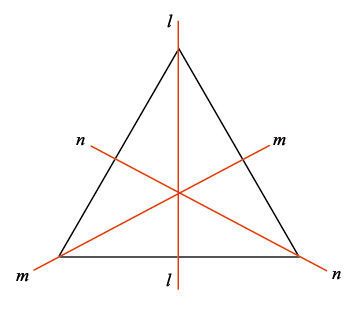
\includegraphics[width=0.5\textwidth]{trougao}
\caption{Симетрије једнакостраничног троугла}
\label{slika:simetrije trougla}
\end{figure}

Као што видимо, постоји 6 трансформација симетрије: \begin{itemize}
                                                         \item Ротације око центра троугла: $r$ (за $\pi/3$), $r\circ r = r^2$ (за $2\pi/3$) и $r\circ r \circ r = r^3 = e$ (за $2\pi$, односно $0$ радијана - идентичко пресликавање)
                                                         \item Осне симетрије $s_1$, $s_2$ и $s_3$ у односу на праве $l$, $m$, $n$ (слика \ref{slika:simetrije trougla}). Приметимо да опет важи $s_i \circ s_i = s_i^2 = e$, за $i\in \lbrace 1, 2, 3 \rbrace$, али и $s_1 s_2 = r^2$, ...
                                                       \end{itemize}
Слично се дешава и код квадрата: он има 4 ротације и 4 осне симетрије. У општем случају, није тешко видети да правилни $n$-тоугао има $2n$ трансформација симетрије: $n$ ротација и $n$ осних симетрија.

Са друге стране, постоје и примери код којих се јавља и транслациона симетрија. Јасно је да то морају бити бесконачни цртежи код којих се један или више основних елементата понављају по једној (\emph{frieze}) или две димензије (\emph{wallpaper}). Интересантно је да се обе врсте оваквих цртежа могу потпуно класификовати у зависности од симетрија које поседују. Тако имамо $7$ frieze-група и $17$ wallpaper-група трансформација.

\begin{figure}[h]
\centering
\begin{subfigure}{0.4\textwidth}
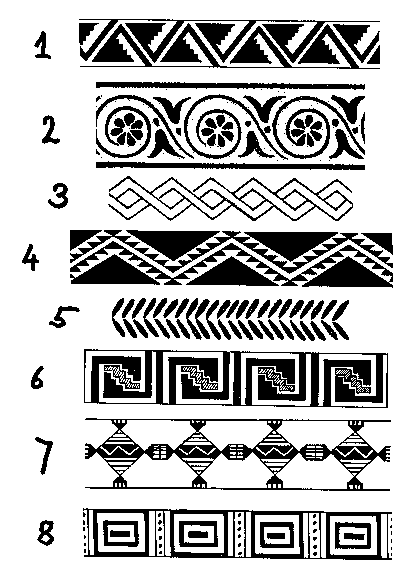
\includegraphics[height=\textwidth]{frieze}
\end{subfigure}
~
\begin{subfigure}{0.4\textwidth}
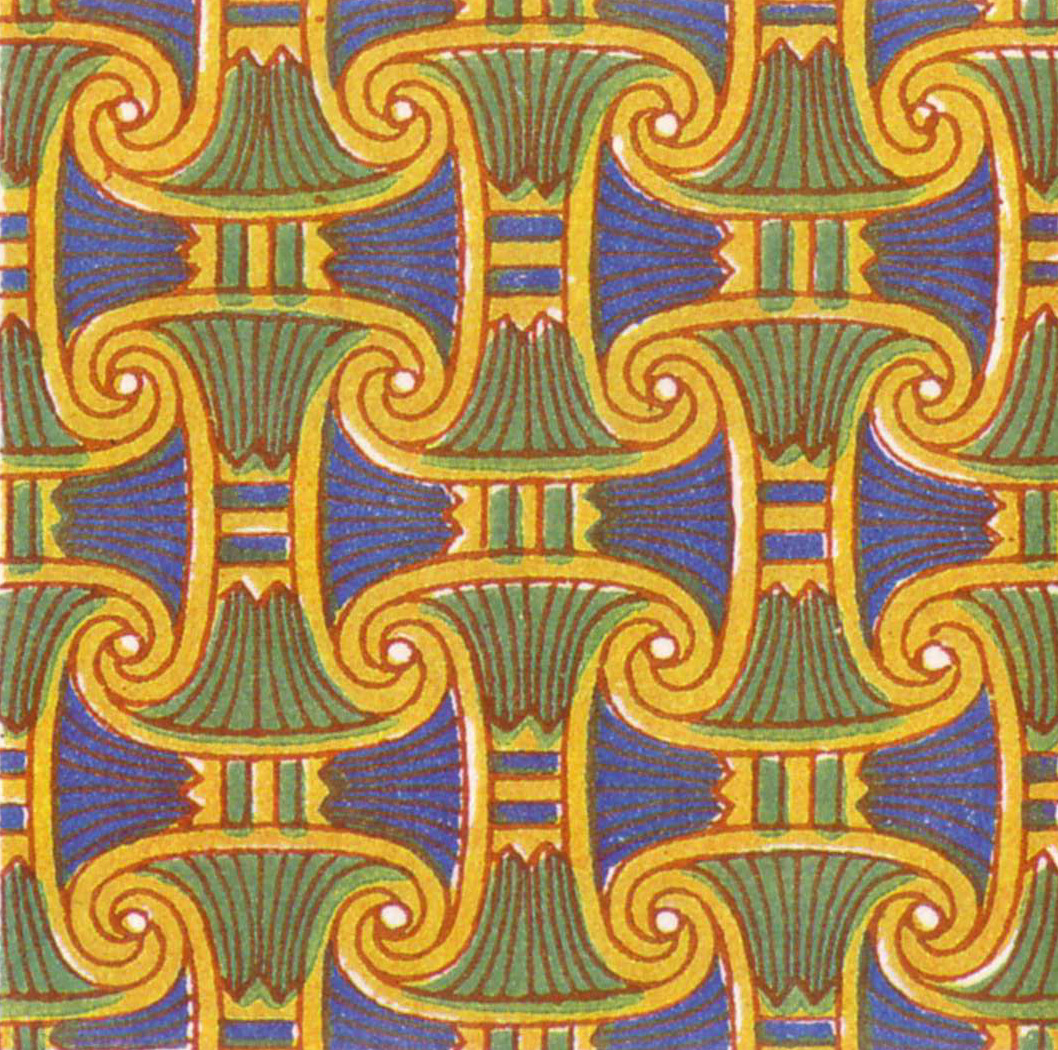
\includegraphics[width=\textwidth]{wallpaper}
\end{subfigure}
\caption{Примери frieze и wallpaper цртежа}
\end{figure}

У три димензије, добро су познате симетрије правилних полиедара (тетраедра, коцке, октаедра, икосаедра и додекаедра), али су значајне и групе симетрија молекула и кристала (кристалографске групе), које се такође могу комплетно класификовати, као у дводимензионалном случају.

\begin{figure}[h]
\centering
\begin{subfigure}{0.3\textwidth}
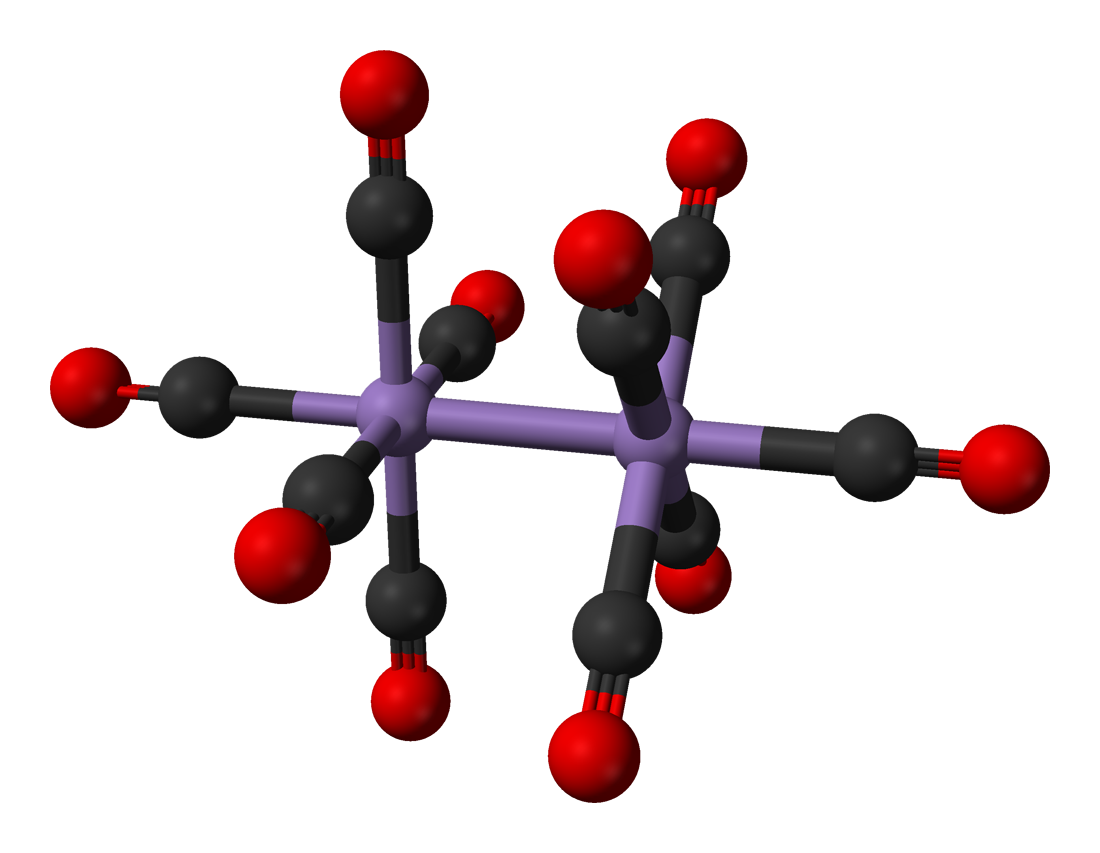
\includegraphics[width=\textwidth]{molekul3}
\caption{Молекул диманган декакарбонила}
\end{subfigure}
~
\begin{subfigure}{0.3\textwidth}
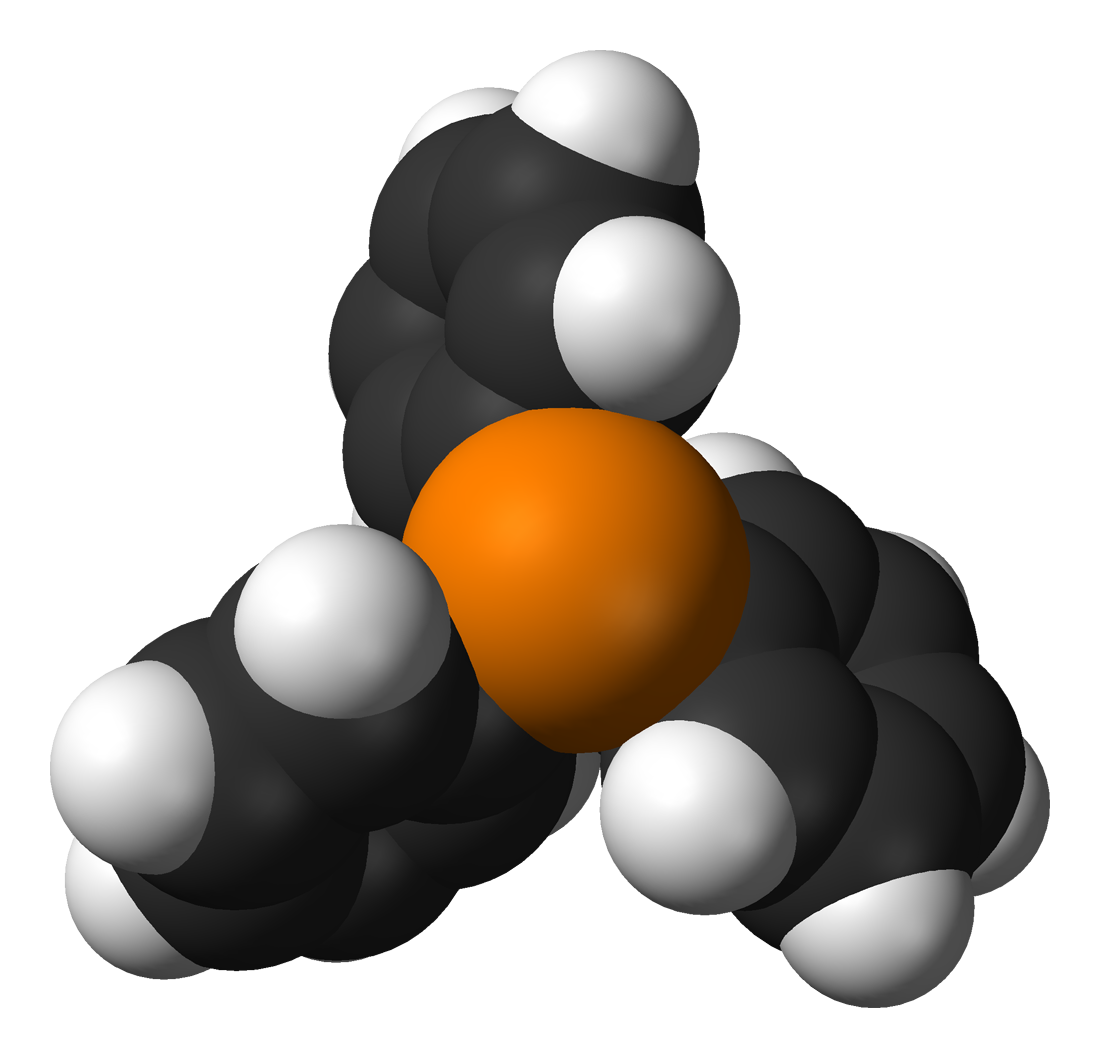
\includegraphics[width=\textwidth]{molekul1}
\caption{Молекул трифенилфосфина}
\end{subfigure}
~
\begin{subfigure}{0.3\textwidth}
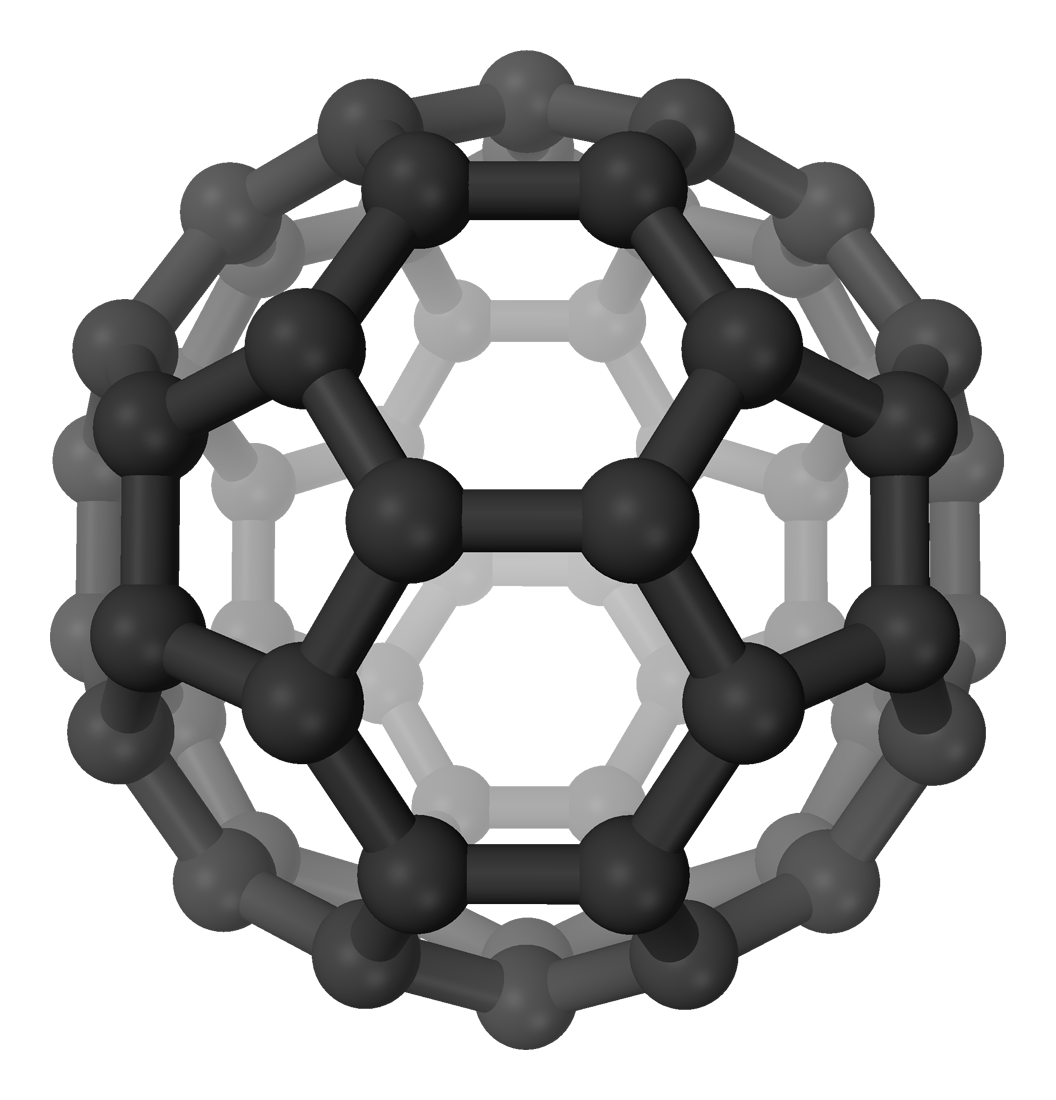
\includegraphics[width=\textwidth]{molekul2}
\caption{Молекул фулерена}
\end{subfigure}
\end{figure}

\begin{figure}[h]
\centering
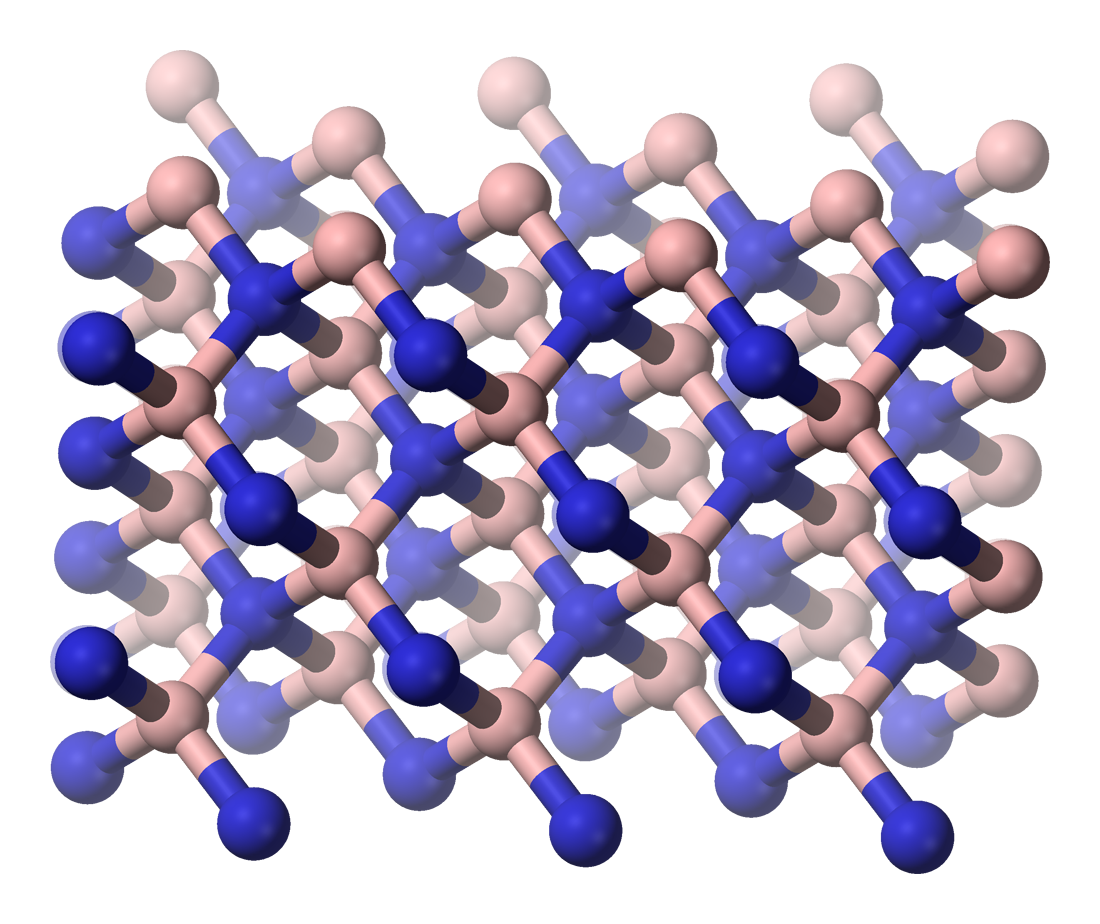
\includegraphics[width=\textwidth]{resetka}
\caption{Кристална решетка коцкастог бор нитрида}
\end{figure}

Циљ овог рада је да покаже колико важну улогу играју симетрије (односно групе као њихова апстракција) у физици. На пример, симетрије нашег простора (Poincaré-ова и Lorentz-ова група у специјалној теорији релативности) произилазе из свих квантних теорија поља, док је сам Стандардни Модел (најприхваћенија таква теорија) базиран на унутрашњим симетријама групе $SU(3)\times SU(2)\times U(1)$.

\chapter{Увод у теорију група}
\section{Основне дефиниције}
%Definicija grupe, red grupe, red elementa, podgrupe.
Као што је већ било речено, елементи неке групе не морају нужно да буду трансформације, већ елементи произвољног скупа $G$, за које смо дефинисали операцију ''множења'' (формално: операцију групе) која задовољава следеће особине:
\begin{enumerate}
  \item Ако $a$ и $b$ припадају $G$, онда и њихов производ, $ab$ припада $G$
  \item Операција множења је асоцијативна, односно важи $a(bc) = (ab)c$
  \item $G$ садржи \emph{јединични елемент} $e$, за који важи $ae = ea = a$, за свако $a\in G$
  \item За свако $a\in G$ постоји $b\in G$, за које важи $ab = ba = e$. Такав $b$ се зове \emph{инверзни елемент} за $a$, и обележава се са $a^{-1}$
\end{enumerate}
У овом тренутку је корисно доказати да је јединични елемент јединствен, као и да за сваки елемент групе постоји јединствен инверзни елемент (иначе ознака $a^{-1}$ не би имала смисла). Претпоставимо дакле супротно, да постоје бар два различита јединична елемента, $e_1$ и $e_2$. Са једне стране, њихов производ је $e_1 e_2 = e_1$, а са друге стране, $e_1 e_2 = e_2$. Ово је контрадикција, дакле, постоји јединствен јединични елемент.

Докажимо сада да је инверзни елемент јединствен. Опет, претпоставимо супротно, да за неки елемент $a$ постоје бар два различита инверзна елемента, $b$ и $b'$. Али, када то распишемо,
$$b = be = b(ab') = (ba)b' = eb' = b',$$
опет долазимо до контрадикције, јер смо претпоставили да је $b\neq b'$. Дакле, за сваки елемент неке групе постоји јединствен њему инверзни елемент.

Иако операцију групе често називамо ''множењем'', она заправо и може а и не мора то да буде:
\begin{itemize}
  \item Скуп рационалних (или реалних) бројева без $0$ чини групу у односу на множење (у уобичајеном смислу)
  \item Скуп целих (али не и природних!) бројева чини групу у односу на сабирање
  \item Скуп свих инвертибилних (регуларних, њихова детерминанта је различита од $0$) квадратних матрица, над пољем $\mathbb{R}$ или $\mathbb{C}$, димензија $n\times n$, чини групу, а операција групе је множење матрица.
\end{itemize}
Али, чак и у овим примерима нисмо причали о апстрактим групама, него о њиховим конкретним примерима, реализацијама. Структура неке апстрактне групе је задата искључиво дефинисањем операције множења сваког уређеног пара елемената, било набрајањем или на неки други начин, али без позивања на ''природу'' тих елемената.\\
Приметимо да операција множења не мора бити комутативна (нпр код множења матрица), али ако јесте, односно ако за свако $a, b\in G$ важи $ab = ba$, онда је група $G$ комутативна или \emph{Абелова}.\\
Број елемената у групи назива се \emph{ред групе}.\\
Ако одаберено неки елемент $a$ групе $G$, можемо га помножити са самим собом и добити производ $aa$, који ћемо обележавати са $a^2$. У општем случају, производ $$\underbrace{aa...a}_{n\text{ пута}}$$ обележавамо са $a^n$. Слично, можемо дефинисати и негативне степене $a$:
$$a^{-n} = (a^{-1})^n = (a^n)^{-1}$$
Ако су сви степени $a$ различити, кажемо да је $a$ \emph{бесконачног реда}. Иначе, исписивањем степена $a$, наићи ћемо на два природна броја $r$ и $s$, $r>s$, за које важи
$$a^r = a^s.$$
Множењем обе стране једнакости са $a^{-s}$, добијамо
$$a^{r-s} = a^0 = e, r-s>0.$$
Нека је $n$ најмањи број за који је $a^n = e$, $n>0$. Тада је $n$ \emph{ред елемента $a$}.

Непразан подскуп $H$ групе $G$ је \emph{подгрупа} групе $G$, ако је $H$ група у односу на рестрикцију операције групе $G$ на скупу $H$. Свака група $G$ са јединичним елементон $e$ има \emph{тривијалне подгрупе} $\{e\}$ и $G$.

Нека је $A$ непразан подскуп групе $G$. Обележимо са $\langle A\rangle$ пресек свих подгрупа $G$ које садже скуп $A$. Пошто се може показати да је пресек две подгрупе неке групе и даље подгрупа те групе, и $\langle A\rangle$ је подгрупа групе $G$. Јасно је да је $\langle A\rangle$ најмања подгрупа $G$ која садржи скуп $A$.

Нека је $\emptyset \neq A\subset G$. Тада подгрупу $\langle A\rangle$ зовемо \emph{подгрупа генерисана скупом $A$}. Ако је $\langle A\rangle=G$, онда скуп $A$ називамо \emph{генераторни скуп} групе $G$, а његове елементе \emph{генератори} групе $G$.

\section{Групе реда 1, 2, 3, 4}

Сада, када смо дефинисали неке основне појмове из теорије група, можемо класификовати све групе реда 1, 2, 3 и 4, као пример.

Група реда 1 садржи само један елемент, и то мора бити јединични елемент $e$, за који важи $ee=e$.

Група реда 2 такође садржи јединични елемент $е$, и још један елемент $a\neq e$. Остаје да видимо чему је једнако $aa$, односно $a^2$. Пошто група има само 2 елемента, или је $a^2 = a$ или је $a^2=e$. У првом случају долазимо до контрадикције, јер би добили да је $a=e$. Дакле, остаје $a^2=e$, односно $a=a^{-1}$. Примери ове групе су
\begin{itemize}
  \item Бројеви 0 и 1, при чему је операција групе сабирање по модулу 2.
  \item Бројеви 1 и -1, при чему је операција групе множење
  \item Јединична трансформација ($e$) и раванска симетрија тродимензионалног еуклидског простора ($a$). Операција групе је композиција две трансформације
  \item Слично као претходно, само што је $a$ централна симетрија у односу на координатни почетак
  \item Слично као претходно, само што је $a$ ротација око неке осе, на пример $z$, за $180^\circ$
\end{itemize}
Као што се види, све ове групе имају у основи исту структуру, и за њих кажемо да су \emph{изоморфне}.

\begin{defn}
У општем случају, кажемо да су две групе $G$ и $H$ изоморфне, ако постоји бијективно пресликавање $\varphi: G\to H$, које има особину да за свако $a, b\in G$ важи $$\varphi(ab) = \varphi(a)\varphi(b)$$
Приметимо овде да производ $ab$ рачунамо у групи $G$, а производ $\varphi(a)\varphi(b)$ према правилима групе $H$.
\end{defn}

Посматрајмо сада групу реда 3, нека су њени елементи $e, a, b$. Слично као у случају групе реда 2, производи $ab$ и $ba$ не могу бити ни $a$ ни $b$, јер би тада било $a=e$ или $b=e$. Дакле, $ab = ba = e$. Елемент $a^2$ не може бити ни $a$ ни $e$, него само $b$. Тако добијамо да су елементи ове групе заправо $a$, $a^2$ и $a^3 = e$. То је пример \emph{цикличне групе} (реда 3 у овом случају), која је генерисана само једним елементом. Таква група постоји за произвољан природан број $n$, обележава се са $C_n$ (циклична група реда $n$), и њени елементи су $\{a, a^2, ..., a^n = e\}$.

Да бисмо олакшали себи посао око представљања неке групе, уобичајено је њене елементе записати у (Кејлијеву) таблицу групе, својеврсне таблице множења за ту групу. На пример, за $C_3$ имамо:\\

\begin{tabular}{c|c c c}
      & $e$ & $a$ & $b(=a^2)$ \\ \hline
  $e$ & $e$ & $a$ & $b$ \\
  $a$ & $a$ & $b$ & $e$ \\
  $b$ & $b$ & $e$ & $a$ \\
\end{tabular}\\

Приметимо да су сви елементи у једној колони и у једној врсти различити, што директно произилази из својства групе (јер би у супротном, за $x\neq y$ имали $ax = ay \Rightarrow a^{-1}ax = a^{-1}ay \Rightarrow x=y$).\\

Коначно, сличним резоновањем долазимо до закључка да постоје две различите, неизоморфне, групе реда 4:
\begin{enumerate}
  \item Циклична група реда 4, $C_4$ :
  \begin{tabular}{c|c c c c}
      & $e$ & $a$ & $b$ & $c$ \\ \hline
  $e$ & $e$ & $a$ & $b$ & $c$ \\
  $a$ & $a$ & $b$ & $c$ & $e$ \\
  $b$ & $b$ & $c$ & $e$ & $a$ \\
  $c$ & $c$ & $e$ & $a$ & $b$ \\
  \end{tabular}
  \item Клајнова 4-група, $V$ :
  \begin{tabular}{c|c c c c}
      & $e$ & $a$ & $b$ & $c$ \\ \hline
  $e$ & $e$ & $a$ & $b$ & $c$ \\
  $a$ & $a$ & $e$ & $c$ & $b$ \\
  $b$ & $b$ & $c$ & $e$ & $a$ \\
  $c$ & $c$ & $b$ & $a$ & $e$ \\
  \end{tabular}
\end{enumerate}

\section{Симетрична група $S_n$, пермутације}
\emph{Пермутације} скупа $\{1, 2, ..., n\}$ су све функције $\pi$ које бијективно пресликавају тај скуп у самог себе. Уобичајено је да се пермутација записује на следећи начин:
$$\pi = \begin{pmatrix}
            1 & 2 & ... & n \\
            a_1 & a_2 & ... & a_n
        \end{pmatrix}$$
при чему је $\{a_1, a_2, ..., a_n\} = \{1, 2, ..., n\}$, и $\pi(i) = a_i$, за $1\leq i\leq n$. Пошто је композиција две бијекције (пермутације) бијекција (пермутација), и пошто за свако пермутацију постоји њој инверзна пермутација, можемо закључити да све ове пермутације једног скупа чине групу (у односу на операцију композиције ових функција-пермутација), и та група се назива \emph{симетрична група скупа од $n$ елемената}, и обележава се са $S_n$.

Са друге стране, посматрајмо неку конкретну пермутацију, на пример:
$$\pi = \begin{pmatrix}
    1 & 2 & 3 & 4 & 5 & 6 & 7 & 8 \\
    2 & 3 & 1 & 5 & 4 & 7 & 6 & 8
  \end{pmatrix},$$
видимо да се 1 слика у 2, затим 2 у 3, и 3 опет у 1. Ови бројеви на тај начин формирају \emph{циклус}, који записујемо као $(123)$. Слично, 4 и 5 формирају циклус $(45)$, 6 и 7 формирају циклус (67), и број 8 формира циклус од једног елемента, $(8)$. Сада ову пермутацију можемо да запишемо на алтернативан начин, као:
$$(123)(45)(67)(8)$$
Приметимо да су сви ови циклуси дисјунктни. Даље, записивање ове пермутације као неког ''производа'' заиста има смисла, ако саме циклусе посматрамо као пермутације, а њихов ''производ'' као композицију тих пермутација. И заиста, за циклус $(123)$ имамо пермутацију
$$\begin{pmatrix}
    1 & 2 & 3 & 4 & 5 & 6 & 7 & 8 \\
    2 & 3 & 1 & 4 & 5 & 6 & 7 & 8
  \end{pmatrix},$$
за циклусе $(45)$ и $(67)$ пермутације
$$\begin{pmatrix}
    1 & 2 & 3 & 4 & 5 & 6 & 7 & 8 \\
    1 & 2 & 3 & 5 & 4 & 6 & 7 & 8
  \end{pmatrix} \text{ и }
  \begin{pmatrix}
    1 & 2 & 3 & 4 & 5 & 6 & 7 & 8 \\
    1 & 2 & 3 & 4 & 5 & 7 & 6 & 8
  \end{pmatrix},$$
и за циклус $(8)$ идентичну пермутацију
$$\begin{pmatrix}
    1 & 2 & 3 & 4 & 5 & 6 & 7 & 8 \\
    1 & 2 & 3 & 4 & 5 & 6 & 7 & 8
  \end{pmatrix}.$$
Приметимо пар чињеница:
\begin{itemize}
  \item Композиција ових пермутација заиста даје почетну пермутацију, $\pi$
  \item Редослед записивања (дисјунктних) циклуса није битан, односно
  $$(123)(45) = (45)(123)$$
  \item У појединачним циклусима, можемо узети било који елемент као почетни,
  $$(123) = (231) = (312)$$
  \item Циклус $(8)$, односно идентичка пермутација се може изоставити, само треба водити рачуна о броју елемената у тој пермутацији
  \item Број пермутованих елемената је 7, а број независних циклуса (не рачунајући циклусе од једног елемента) је 3. Разлика ова два броја је \emph{декремент пермутације}. Дефинишемо \emph{парност пермутације} као парност декремента.
\end{itemize}

Једна од основних теорема у теорији група је Кејлијева (Cayley) теорема, која гласи овако:
\begin{thm}
Свака група $G$ реда $n$ је изоморфна са подгрупом симетричне групе $S_n$.
\end{thm}
\begin{proof}
Нека је $G = \{a_1, a_2, ..., a_n\}$ . Посматрајмо произвољни елемент $b\in G$, и његове производе $ba_1, ba_2, ..., ba_n$ са свим осталим елементима $G$. Као што смо раније приметили, сви ови производи морају бити различити. Зато, производи $ba_i$ су у ствари нека пермутација скупа $G$:
$$b\to \pi_b = \begin{pmatrix}
                a_1 & ... & a_n \\
                ba_1 & ... & ba_n
               \end{pmatrix}$$
Сличне пермутације можемо придружити и осталим елементима $G$. Пошто желимо да покажемо да постоји изоморфизам између групе $G$ и групе ових пермутација, треба да покажемо да ће за произвољно $b, c\in G$ пермутација $\pi_c \pi_b$ заиста одговарати елементу $cb$. Посматрајмо дакле пермутацију $\pi_c$:
$$\pi_c = \begin{pmatrix}
                a_1 & ... & a_n \\
                ca_1 & ... & ca_n
          \end{pmatrix}$$
Она се може написати и на други начин, као
$$\pi_c = \begin{pmatrix}
                ba_1 & ... & ba_n \\
                c(ba_1) & ... & c(ba_n)
          \end{pmatrix}$$
Сада лако можемо добити производ $\pi_c \pi_b$:
$$\pi_c \pi_b= \begin{pmatrix}
                ba_1 & ... & ba_n \\
                c(ba_1) & ... & c(ba_n)
               \end{pmatrix}
               \begin{pmatrix}
                a_1 & ... & a_n \\
                ba_1 & ... & ba_n
               \end{pmatrix}$$
Множењем ове две пермутације добијамо
$$\pi_c \pi_b= \begin{pmatrix}
                a_1 & ... & a_n \\
                cba_1 & ... & cba_n
               \end{pmatrix} = \pi_{cb}$$

Дакле, тражени изоморфизам $\varphi: G\to S_n$ је $\varphi(a) = \pi_a$.
\end{proof}
Ова теорема нам показује да постоји коначан број група реда $n$, и даје нам систематичан начин за налажење сви тих група (све подгрупе $S_n$).

\section{Лагранжова теорема}
Још једна теорема корисна за одређивање структура свих модућих група датог реда, али и за многе друге проблеме, је Лагранжова (Lagrange) теорема.
\begin{thm}
Ако је $G$ нека група реда $n$, и $H$ њена подгрупа реда $m$, тада $m$ дели $n$.
\end{thm}
\begin{proof}
Ако је $H=G$, тврђење је тривијално тачно. Иначе, постоји неки елемент $a\in G$, тако да $a\notin H$. Ако обележимо елементе подгрупе $H$ са $e, h_2, ..., h_m$, тада дефинишемо скуп $aH$ као скуп производа $a$ и свих елемената групе $H$,
$$aH = \{a, ah_2, ..., ah_m\}.$$
Због особина групе имамо да су сви $ah_i$ различити (иначе би постојало $j, j\neq i$, за које је $h_i=h_j$), као и да је $aH\cap H = \emptyset$ (иначе би било и $a\in H$).

Сада имамо два скупа од по $m$ различитих елемената, $H$ и $aH$, који се садрже у $G$. Уколико у $G$ joш постоје елементи који нису ни у $H$, ни у $aH$, понављамо овај поступак за један такав елемент, $b$, и формирамо $bH$. Приметимо да, ако би било $aH\cap bH \not= \emptyset$, тада би постојали $h_1, h_2\in H$, за које би важило $ah_1 = bh_2$. Али, множењем са $h_2^{-1}$ би добили $a(h_1h_2^{-1}) = b$, односно $b\in aH$, што је по конструкцији није тачно. Као резултат, поделили смо групу $G$ на $k$ дисјунктних подскупова:
$$G = H \cup a_1 H \cup a_2 H \cup ... \cup a_{k-1} H.$$
Број $k$ се зове \emph{индекс} подгрупе $H$ у групи $G$. Скупови $a_i H$ се зову \emph{леве класе} $H$ у $G$, а скуп свих левих класа неке подгрупе се обележава са $G/H$. Приметимо да смо на сличан начин могли да поделимо $G$ и на \emph{десне класе}:
$$G = H \cup Ha_1'  \cup Ha_2' \cup ... \cup Ha_{k-1}'.$$
\end{proof}
\begin{cor}
Ред елемента (цикличне подгрупе генерисане тим елементом) дели ред групе.
\end{cor}

\section{Инваријантне подгрупе, фактор група}
%Konjugacija, unutrasnji automorfizam, invarijantna (normalna) podgrupa, faktor grupa, homomorfizam.
\begin{defn}
За елемент $b$ групе $G$ кажемо да је \emph{конјугован} елементу $a$ ако постоји $u\in G$ за који важи
$$u a u^{-1} = b$$
\end{defn}
Видимо да ако одаберемо $u = e$, добијамо да је $a$ само себи конјуговано. Такође, ако је $b$ конјуговано са $a$, $c$ конјуговано са $b$, тада је и $c$ конјуговано са $a$ (јер је $c = vbv^{-1}$, $b = uau^{-1}$, па је $c = vuau^{-1}v^{-1}$, односно $c = (vu)a(vu)^{-1}$). Коначно, једноставно се види да ако је $u a u^{-1} = b$, тада је и $a = u^{-1} b (u^{-1})^{-1}$.

На овај начин смо утврдили да је релација конјугације рефлексивна, симетрична и транзитивна, дакле - релација еквиваленције. Таква релација разбија скуп на класе еквиваленције, у овом случају \emph{класе конјугације}. Ако је група комутативна, тада сваки елемент чини класу за себе, јер за свако $a, b$, $bab^{-1} = a$.

У случају група трансформација, класе конјугације имају једноставну ''физичку'' интерпретацију, у смислу да групишу ''сличне'' трансформације у једну класу. На пример, ако са $r$ обележимо неку ротацију, а са $s$ неку осну симетрију са осом која пролази кроз центар ротације $r$, тада је $r s r^{-1}$ трансформација осне симетрије у односу на неку нову осу, насталу ротацијом осе $s$ за $r$. Касније ћемо видети да две матрице припадају истој класи конјугације ако и само ако представљају исту линеарну трансформацију, записану у различитим базама.

Посматрајмо подгрупу $H$ групе $G$. Тада се лако показује да је и $aHa^{-1}$ (сви производи $aha^{-1}$, где $h\in H$) подгрупа од $G$, при чему је $a$ произвољни елемент из $G$. Уколико за свако $a\in G$ важи
$$aHa^{-1} = H,$$
тада кажемо да је $H$ \emph{инваријантна} или \emph{нормална подгрупа} групе $G$, и то обележавамо са $H\lhd G$. Последња једнакост у ствари значи да за дати елемент $h_1\in H$, за свако $a\in G$, можемо наћи $h_2\in H$, тако да буде $ah_1a^{-1} = h_2$, односно $ah_1 = h_2 a$, што се може краће записати и као
$$aH = Ha, $$
и тако добијамо алтернативну дефиницију нормалне подгрупе: Подгрупа $H$ је нормална у $G$, ако су лева и десна класа једнаке, без обзира на то са којим елементом из $G$ их формирамо.

Коначно, можемо приметити још један потребан и довољан услов да нека подгрупа буде нормална, а то је да она садржи елементе $G$ у комплетним класама конјугације, тј. садржи или све или ни један елемент из неке дате класе конјугације.

Можда ће се неко запитати чему све ово, али испоставља се да овакве подгрупе имају нека врло интересантна својства. За неку групу $G$ и њену нормалну подгрупу $H$ дефинишимо операцију $\cdot: G/H \to G/H$ као $aH\cdot bH := abH$. Прво, треба показати да резултат не зависи од избора представника класа, односно да ако важи
$$aH = a_1 H \text{ и } bH = b_1 H,$$
тада мора бити $aH\cdot bH = a_1 H \cdot b_1 H$, тј. $abH = a_1 b_1 H$. Докажимо да је $abH \subseteq a_1 b_1 H$ и $a_1 b_1 H \subseteq abH$.

Нека је $x\in abH$. Тада постоји $h\in H$, такво да $x=abh$. Пошто је $bh\in bH$, тада постоји $h_1\in H$, тако да $bh = b_1 h_1$. Дакле,
$$x = abh = ab_1 h_1.$$
Како је $H\lhd G$, $b_1 H = Hb_1$, па онда $(\exists h_2\in H)(b_1h_1=h_2b_1)$. Таквим резоновањем добијамо
$$x = ab_1h_1 = ah_2b_1 = a_1h_3b_1 = a_1b_1h_4 \in a_1b_1H.$$

Дакле $x\in abH \Rightarrow x\in a_1b_1H$, па  је $abH \subseteq a_1b_1H$. Други смер, $a_1 b_1 H \subseteq abH$ се показује аналогно, па коначно имамо $abH = a_1b_1H$.

Показали смо да је операција $(aH)\cdot (bH) = (ab)H$ добро дефинисана. Није тешко доказати да је скуп свих левих класа $G/H$ (у случају да је $H\lhd G$) група у односу на овако дефинисану операцију. Јединични елемент је $eH = H$, а инверзни елемент за класу $aH$ је:
$$(a^{-1}H)(aH) = a^{-1}HaH = a^{-1}aHH = H.$$

Овако добијена група се назива \emph{фактор-група}, обележава се са $G/H$. Приметимо да је њен ред индекс групе $H$ у $G$.

\chapter{Векторски простори}
За примену теорије група у физици потребно је дефинисати још и појам векторског простора (што је заправо уопштење свима добро познатог еуклидског простора). Након тога ћемо моћи да посматрамо неке групе као групе трансформација векторских простора.
\section{Основне дефиниције}
Нека је $(V, +)$ комутативна група, а $(F, +, \cdot)$ поље. $V$ је \emph{векторски простор над пољем} $F$, ако је дефинисано пресликавање $F\times V\to V$, при чему слику пара $(\alpha, v)$ означавамо са $\alpha v$, тако да за свако $\alpha, \beta \in F$, $u, v\in V$ важи:
\begin{enumerate}
\item $\alpha(u+v) = \alpha u+\alpha v$
\item $(\alpha + \beta)v = \alpha v+ \beta v$
\item $(\alpha\cdot\beta)v = \alpha(\beta v)$
\item $1v = v$
\end{enumerate}
где је са $1$ означен неутрални елеменат за множење поља $F$. Елементи скупа $F$ се називају \emph{скалари}, а елементи скупа $V$ - \emph{вектори}. Ми ћемо у овом раду посматрати искључиво поља реалних и комплексних бројева.

На пример, $\mathbb{R}^n$ је векторски простор над $\mathbb{R}$, при чему је сабирање $n$-торки, односно множење $n$-торке реалним бројем дефинисано по-елементно.

Други пример је $\mathbb{R}[x]$, скуп свих полинома са реалним коефицијентима над пољем $\mathbb{R}$. Операција сабирања вектора је сабирање полинома, а множење скаларом - множење сваког коефицијента полинома тим скаларом.

У векторском простору $V$, вектор $v$ је \emph{линеарна комбинација} вектора $v_1, ..., v_n$ ако постоје скалари $\alpha_1, ...\alpha_n$ такви да је $$v = \alpha_1 v_1+ \alpha_2 v_2+ \cdots+\alpha_n v_n$$

Ако је $S\subseteq V$, са $L(S)$ обележавамо скуп свих линеарних комбинација вектора из $S$. Кажемо да скуп вектора $S\subset V$ \emph{генерише} векторски простор $V$, ако је $V = L(S)$.

У векторском простору $V$ скуп вектора $v_1, ...,v_n$ је \emph{линеарно зависан}, ако постоје скалари $\alpha_1, ...,\alpha_n$, од којих је бар један различит од нуле, такви да је $$\alpha_1 v_1 + \alpha_2 v_2 + \cdots+\alpha_n v_n = 0.$$ Низ вектора који није линеарно зависан је \emph{линеарно независан}.
\emph{База} векторског простора је низ вектора који је линеарно независан и који генерише векторски простор.
На пример, вектори $(1, 0, 0)$, $(0, 1, 0)$ и $(0, 0, 1)$ су база векторског простора $\mathbb{R}^3$.
Може се показати да постоји још еквивалентних дефиниција, односно потребних и довољних услова да би неки низ вектора био база. Наводимо их овде, јер ће бити корисне у даљем тексту:
\begin{itemize}
  \item У векторском простору $V$ низ вектора је база ако и само ако је тај скуп максималан линеарно независан скуп.
  \item У векторском простору $V$ низ вектора је база ако и само ако је тај скуп минималан скуп генератора
  \item У векторском простору $V$ низ вектора $v_1, ..., v_n$ је база ако и само ако се сваки вектор $x\in V$ може на јединствен нечин написати у облику $$x = \sum_1^n\alpha_i v_i, \quad \alpha_1, ..., \alpha_n\in F$$
\end{itemize}
Одавде се може наслутити да све базе неког одређеног векторског простора $V$ имају исти број елемената, што се може и показати, а тај број се зове \emph{димензија векторског простора}, и обележава се са $\operatorname{dim} V$.

На пример, векторски простор $\mathbb{R}^n$ има димензију $n$, док векторски простор реалних полинома $\mathbb{R}[x]$ има бесконачну димензију.

У даљем тексту ћемо се фокусирати на коначно-димензионалне векторске просторе.

\section{Унитарни векторски простори}

Нека је $V$ векторски простор над пољем $F$ (где је $F=\mathbb{R}$ или $F=\mathbb{C}$). \emph{Унутрашњи (скаларни) производ} на $V$ је свака функција $(,):V\times V\to F$, при чему слику уређеног пара вектора $(x, y)\in V\times V$ означавамо са $(x, y)$, за коју за свако $x, y, z\in V$ и свако $\alpha \in F$ важи
\begin{enumerate}
  \item $(x, y) = \overline{(y, x)}$
  \item $(x+y, z) = (x, z)+(y, z)$
  \item $(\alpha x, y) = \alpha (x, y)$
  \item $(x, x)\geq 0$
  \item $(x, x) = 0 \Leftrightarrow x=0$
\end{enumerate}
Са $\overline{(x, y)}$ означен је комплексан број конјугован са $(x, y)$. Приметимо да је $(x, x) = \overline{(x, x)} \Rightarrow (x, x)\in \mathbb{R}$, па је услов $(x, x)\geq 0$ добро дефинисан.

Векторски простор над пољем реалних или комплексних бројева заједно са функцијом која дефинише унутрашњи производ назива се \emph{унитарни векторски простор}.

Специјално, \emph{еуклидски векторски простор} је унитарни векторски простор над пољем реалних бројева.

Један пример унитарног векторског простора је $\mathbb{R}^n$, заједно са \emph{стандардним скаларним производом} вектора $x = (x_1, ..., x_n)$, $y = (y_1, ..., y_n)$:
$$(x, y) = \sum_{i=1}^{n} x_iy_i$$

Такође, у векторском простору $\mathbb{R}^2$ свака бинарна операција дефинисана са
$$(x, y) = x_1y_1 - x_1y_2 - x_2y_1 +ax_2y_2,$$
где је $a>1$, јесте скаларни производ. Према томе, од векторског простора $\mathbb{R}^2$ се може добити бесконачно много различитих еуклидских простора.

У унитарном векторском простору $V$ функција $\|\;\|:V\to \mathbb{R}$, дефинисана са $$\|x\| = \sqrt{(x, x)}$$ назива се \emph{норма} на $V$. Ненегативан реалан број $\|x\|$ назива се \emph{норма вектора} $x$.
\emph{Растојање} вектора $x$ и $y$ је дефинисано са $$d(x, y) = \|x-y\|.$$

Позната Коши-Шварцова неједнакост важи у било ком унитарном векторском простору:
\begin{thm}
У унитарном векторском простору $V$ за свако $x, y\in V$ важи
$$|(x, y)|\leq\|x\|\|y\|,$$
при чему једнакост важи ако и само ако су вектори $x$ и $y$ линеарно зависни. (Са $|(x, y)|$ смо обележили модуо комплексног броја $(x, y)$)
\end{thm}
Као последицу, у еуклидским векторским просторима можемо дефинисати угао између вектора $x\neq 0$ и $y\neq 0$, као реалан број $\alpha\in [0, \pi]$, такав да је $$\cos \alpha = \frac{(x, y)}{\|x\|\|y\|}$$
Природно, за два вектора $x$ и $y$ кажемо да су \emph{ортогонални} ако је $(x, y) = 0$.

Такође, из дефиниције унутрашњег производа добијамо корисно својство да за $x\in V, \alpha \in F$ важи $\|\alpha x\| = |\alpha|\; \|x\|$.

За базу $B=\{b_1, ..., b_n\}$ неког унитарног векторског простора $V$ кажемо да је \emph{ортонормирана}, ако је
$$(b_i, b_j) = \begin{cases}
                1 & \mbox{ако } i=j \\
                0 & \mbox{ако } i\neq j
               \end{cases}$$
Сваки унитарни векторски простор поседује бар једну ортонормирану базу, и она се може добити из произвољне базе применом \emph{Грам-Шмитовог поступка}\cite{milic}.

\section{Линеарне трансформације}
Сад, кад смо дефинисали неке основне појмове везане за векторске просторе, можемо наставити са дефинисањем линеарних трансформација и њихове везе са матрицама.
\begin{defn}
Нека су $V_1$ и $V_2$ векторски простори над истим пољем $F$. Пресликавање $A: V_1\to V_2$ такво да је
$$(\forall a, b\in V_1)(\forall \alpha, \beta \in F) A(\alpha a+ \beta b) = \alpha A(a) + \beta A(b)$$
назива се \emph{линеарна трансформација (линеарни оператор, хомоморфизам)} векторског простора $V_1$ у $V_2$. Уколико је $V_1 = V_2 = V$, тада је $A$ просто линеарна трансформација векторског простора $V$.
\end{defn}
Значајно је да је свака линеарна трансформација на јединствен начин одређена ако је познато како се пресликавају вектори базе, што нам омогућава да представимо произвољну линеарну трансформацију неког коначно димензионалног векторског простора помоћу матрице, на следећи начин:\\
Претпоставимо да је $\{a_1, ...a_n\}$ база векторског простора $V$. Тада, линеарну трансформацију $A$ можемо задати са
$$A(a_1) = b_1, A(a_2) = b_2, ..., A(a_n) = b_n$$
где су $b_1, ..., b_n\in V$. Пошто је $\{a_1, ...a_n\}$ база, сваки од вектора $b_i$ може се на јединствен начин написати као линеарна комбинација вектора базе, па имамо:
$$A(a_1) = \alpha_{11}a_1 + \alpha_{21}a_2 + ... + \alpha_{n1}a_n$$
$$A(a_2) = \alpha_{12}a_1 + \alpha_{22}a_2 + ... + \alpha_{n2}a_n$$
$$...$$
$$A(a_n) = \alpha_{1n}a_1 + \alpha_{2n}a_2 + ... + \alpha_{nn}a_n$$
Ове коефицијенте можемо записати и у компактнијем облику, као матрицу:
$$[A] = \begin{bmatrix}
    \alpha_{11} & \alpha_{12} & ... & \alpha_{1n} \\
    \alpha_{21} & \alpha_{22} & ... & \alpha_{2n} \\
    ... & ... & ... & ... \\
    \alpha_{n1} & \alpha_{n2} & ... & \alpha_{nn}
  \end{bmatrix},$$
па вредност функције $A(x)$ (као линеарне трансформације произвољног вектора $x\in V$) можемо израчунати простим множењем матрица:
$$[A(x)] = [A][x] = \begin{bmatrix}
            \alpha_{11} & \alpha_{12} & ... & \alpha_{1n} \\
            \alpha_{21} & \alpha_{22} & ... & \alpha_{2n} \\
            ... & ... & ... & ... \\
            \alpha_{n1} & \alpha_{n2} & ... & \alpha_{nn}
           \end{bmatrix}
           \begin{bmatrix}
           \zeta_1\\
           \zeta_2\\
           \vdots \\
           \zeta_n
           \end{bmatrix}
$$
при чему је $x = \zeta_1 a_1 + \zeta_2 a_2 + ... \zeta_n a_n$. Слично, може се показати да се и композиција линеарних трансформација може представити множењем одговарајућих матрица (које морају да се односе на исту базу), тј. $[AB] = [A][B]$.

Приметимо да матрични запис линеарне трансформације зависи од избора базе:\\
Нека су $B_1$ и $B_2$ две различите базе коначнодимензионалног векторског простора, и $P$ и $Q$ матрице једне исте линеарне трансформације, записане у базама $B_1$ и $B_2$, редом. Тада се може доказати да постоји матрица $S$, таква да важи
$$P = SQS^{-1}.$$

\chapter{Групе у физици}

\section{Групе матрица}

Наведимо прво неке од најчешће коришћених класа група у физици (а и шире):

\begin{enumerate}
  \item \emph{Општа линеарна група, $GL(n, \mathbb{C})$} скуп свих $n\times n$ регуларних (инвертибилних, детерминанта различита од 0) матрица над $\mathbb{C}$, у односу на множење матрица. Ове матрице одговарају свим инвертибилним линеарним трансформацијама простора $\mathbb{C}^n$. Њена подгрупа је $GL(n, \mathbb{R})$, скуп свих инвертибилних реалних матрица $n\times n$ у односу на множење.
  \item \emph{Специјална линеарна група}, $SL(n, \mathbb{C}) = \{M\in GL(n, \mathbb{C})|\det M = 1\}$. Слично,
  $$SL(n, \mathbb{R}) = \{M\in GL(n, \mathbb{R})|\det M = 1\}.$$
  \item \emph{Унитарна група, $U(n)$}
  $$U(n) = \{M\in GL(n, \mathbb{C})|MM^\dag = I\},$$
  где $U^\dag$ означава \emph{транспоновани конјугат} матрице $U$, и добија се транспоновањем матрице $U$, и конјуговањем свих њених елемената. Важно својство унитарних матрица је да, уколико их интерпретирамо у односу на неку ортонормирану базу као операторе над комплексним векторским простором $\mathbb{C}^n$, оне чувају скаларни производ вектора свих вектора $x = (x_1, ..., x_n)$, $y = (y_1, ...y_n)$:
  $$(Mx, My) = (x, y) = \sum_{i=1}^n x_i \overline{y}_i.$$
  Подгрупа ове групе је \emph{специјална унитарна група},
  $$SU(n) = \{M\in U(n)|\det M = 1\}.$$
  \item \emph{Ортогонална група, $O(n)$}
  $$O(n) = \{M\in GL(n, \mathbb{R})|MM^T = 1\}.$$
  Слично као унитарна група, уколико њене елементе интерпретирамо у односу на неку ортонормирану базу као операторе над еуклидским просторима, оне чувају стандардни скаларни производ
  $$(Mx, My) = (x, y) = \sum_{i=1}^n x_i y_i.$$
  Даље, \emph{специјална ортогонална} група је дефинисана са
  $$SO(n) = \{M\in O(n)|\det M = 1\}.$$
  \item \emph{Псеудоортогонална група, $O(p, q)$} Нека је $g$ дијагонална матрица $g = \operatorname{diag}(\underbrace{1, .., 1}_p, \underbrace{-1, ..., -1}_q)$. Псеудоортогонална група $O(p, q)$ се дефинише као
      $$O(p, q) = \{M\in GL(n, \mathbb{R})|M^TgM = g\}.$$
      Касније, у секцији \ref{dokaz za pseudoortogonalnu kvadratnu formu}, доказаћемо да су то управо матрице које чувају квадратну форму
      $$\sum_{i=1}^p x_iy_i - \sum_{i=1}^q x_{p+i}y_{p+i}.$$
  Најпознатија група ове врсте је Лоренцова група $O(1, 3)$, са којом ћемо се позабавити на крају овог рада.
\end{enumerate}

\section{Симетрије унитарних векторских простора}
\label{simetrije unitarnih prostora}

Пре него што пређемо на разматрање групе Лоренцових трансформација, размотримо везу између изометрија еуклидских простора и трансформација које чувају скаларни производ.

\begin{defn}
Нека је дат еуклидски векторски простор $V$ коначне димензије.
\begin{description}
  \item[Изометријске трансоформације] су трансформације (пресликавања) $M: v\to V$, које чувају растојање, тј. за свако $u,v$ важи
  $$\|u-v\| = \|M(u)-M(v)\|$$
  \item[Ортогоналне трансформације] су трансформације $M: V\to V$ које чувају скаларни производ, тј.
  $$(u, v) = (M(u), M(v))$$
\end{description}
\end{defn}

Следеће две теореме објашњавају односе између ортогоналних и изометријских трансформација.
\begin{thm}
Нека је $M:V\to V$ ортогонално пресликавање еуклидског векторског простора. Тада је $M$ изометријска трансформација која чува 0, тј. $M(0) = 0$.
\end{thm}
\begin{proof}
Знамо да пошто $M$ чува скаларни производ, и дужина произвољног вектора остаје очувана:
$$\|x\|^2 = (x, x) = (M(x), M(x)) = \|M(x)\|^2.$$
Према томе, $\|M(0)\| = \|0\| = 0$, па је $M(0) = 0$.
Докажимо сада да $M$ чува растојање, односно да за свако $a, b\in V$ важи $$\|a-b\| = \|M(a)-M(b)\|.$$
Пошто је норма по дефиницији увек ненегативна, довољно је показати ја је
$$\|a-b\|^2 = \|M(a)-M(b)\|^2.$$
Због билинеарности скаларног производа, можемо доказати уопштење косинусне теореме:
$$\|x-y\|^2 = (x-y, x-y) = (x, x-y)-(y, x-y) = $$
$$ = (x, x) - (x, y) - (y, x) + (y, y) = \|x\|^2 - 2(x, y) + \|y\|^2$$
Даље имамо
$$\|a-b\|^2 = \|a\|^2-2(a, b)+\|b\|^2=\|M(a)\|^2-2(M(a), M(b))+\|M(b)\|^2 = \|M(a)-M(b)\|^2$$
Дакле, $M$ је изометрија.
\end{proof}

\begin{thm}
Нека је $M$ изометрија неког еуклидског векторског простора и нека је $M(0) = 0$. Тада је $M$ ортогонална трансформација
\end{thm}
\begin{proof}
 Нека је $y=0$. Тада је
  $$\|M(x)\| = \|M(x)-0\| = \|M(x)-M(0)\| = \|x-0\| = \|x\|$$
  тј. $\|M(x)\| = \|x\|$. Нека је сад $M(x)=x'$ и $M(y)=y'$. Пошто имамо
  $$\|x'\|=\|x\|,\; \|y'\|=\|y\|,$$
  \begin{equation}\label{eq:izometrija}
  \|x'-y'\|=\|x-y\| \tag{*}
  \end{equation}
  и пошто знамо да важи
  $$\|a-b\|^2 = \|a\|^2 - 2(a, b)+\|b\|^2,$$
  можемо квадрирати \eqref{eq:izometrija} и добити
  $$\|x'\|^2-2(x',y')+\|y'\|^2 = \|x\|^2-2(x, y)+\|y\|^2$$
  односно
  $$(x, y) = (x', y').$$
  Дакле, $M$ чува скаларни производ, па је ортогонална трансформација.
\end{proof}

\begin{lem}
  Нека је $V$ коначнодимензионални еуклидски векторски простор, и $B = (b_1, ..., b_n)$ његова ортонормирана база. Ако су $x, y \in V$, и $x = x_1b_1+...+x_nb_n$, $y = y_1b_1+...+y_nb_n$, нека су $[x], [y]$ вектори колона у тој бази. Тада је $$(x, y) = [x]^T [y] = \sum_{i=1}^{n} x_iy_i$$
\end{lem}
\begin{proof}
    Због билинеарност, имамо
    $$(x, y) = (\sum x_ib_i, \sum y_j b_j) = \sum \sum x_iy_j(b_i, b_j) = \sum x_iy_i, $$
    јер је $(b_i, b_j) = 0$ за $i\neq j$, а $(b_i, b_j) = 1$ за $i=j$.
\end{proof}

Последња теорема у овом одељку говори о још неким својствима ортогоналних трансформација
\begin{thm}
Ако је $M$ ортогонална трансформација коначнодимензионалног еуклидског простора, тада важи
\begin{enumerate}
  \item $M$ је линеарна трансформација
  \item Ако је $[M]$ матрица трансофмрације $M$ у односу на неку ортонормирану базу, тада важи $[M]^T[M] = I$
  \item $M$ је инвертибилна и $M^{-1}$ је такође изометрија
  \item $\det [M]=\pm 1$ (у било којој бази)
\end{enumerate}
\end{thm}
\begin{proof}
\begin{enumerate}
  \item Треба показати да је
  $$M(x+y) = M(x)+M(y), \; M(\alpha x) = \alpha M(x).$$
  Означимо $z = x+y$, $M(x)=x'$, $M(y)=y'$, $M(z)=z'$. Докажимо прво да је
  $$z'-x'-y' = 0 \text{ , тј. } \|z'-x'-y'\|^2 = 0.$$
  Приметимо да за све $x, y, z, x', y', z'$ важи
  $$\|z-x-y\|^2 = \|z\|^2+\|x\|^2+\|y\|^2 - 2(x, y) -2(y, z) - 2(z, x),$$
  $$\|z'-x'-y'\|^2 = \|z'\|^2+\|x'\|^2+\|y'\|^2 - 2(x', y') -2(y', z') - 2(z', x').$$
  Пошто $M$ чува све норме и скаларне производе, добијамо да је
  $$\|z'-x'-y'\|^2 = \|z-x-y\|^2.$$
  Специјално, за $z=x+y$ имамо
  $$\|z'-x'-y'\|^2 = \|z-x-y\|^2 = \|0\|^2 = 0.$$
  Дакле, $M(x+y) = M(x)+M(y)$. Докажимо још да је $M(\alpha x) = \alpha M(x)$, односно слично, $\|M(\alpha x) - \alpha M(x)\|^2 = 0$.
  $$\|M(\alpha x) - \alpha M(x)\|^2 = \|M(\alpha x)\|^2 + \|\alpha M(x)\|^2 - 2(\alpha M(x), M(\alpha x))$$
  $$ = \|\alpha x\|^2 + \alpha^2 \|M(x)\|^2 - 2\alpha(M(x), M(\alpha x))$$
  $$ = \alpha^2\|x\|^2 + \alpha^2 \|x\|^2 - 2\alpha(x, \alpha x)$$
  $$ = 2\alpha^2\|x\|^2 - 2\alpha^2 (x, x) = 0.$$
  Овим смо показали да је $M$ линеарна трансформација.
  \item Како радимо у ортонормираној бази, можемо користити претходну лему:
  $$(x, y) = [x]^TI[y],$$
  $$(M(x), M(y)) = [x]^T[M]^TI[M][y].$$
  Из ортогоналности $M$, добијамо
  $$(x, y) = (M(x), M(y))$$
  $$[x]^T[y] = [x]^T[M]^T[M][y]$$
  $$[x]^T[y] - [x]^T[M]^T[M][y] = 0$$
  $$[x]^T(I-[M]^T[M])[y] = 0.$$
  Пошто ова једнакост важи за све $x, y\in V$, мора бити $[M]^T [M] = I$, што је и требало показати.
  \item Тривијално на основу претходног.
  \item Јасно је да тврђење важи у ортонормираној бази.
  $$1 = \det I = \det([M]^T[M]) = \det [M] \det {[M]^T} = (\det [M])^2$$
  Ако је $Q$ матрица те трансформације у некој другој бази, онда је $Q = S[M]S^{-1}$. Према томе,
  $$\det Q = \det S \det [M] \det S^{-1} = \det [M]$$
\end{enumerate}
\end{proof}

\section{Лоренцове трансформације}

Једна од првих последица специјалне теорије релативности јесте да не постоје апсолутни просторни и временски референтни системи. Другим речима, може се десити да су се, гледано из једног референтног система, два догађаја одиграла истовремено, на различитим местима, док су се у неком другом референтном систему та два догађаја одиграла на истом месту, у различито време.

Испоставља се да простор и време не можемо посматрати одвојено, као и да више не можемо говорити о догађајима који су се одиграли ''на истом месту'' или ''у исто време''. На срећу, математички формализам Минковског нам омогућава да ипак уведемо некакву меру ''удаљености'' између два догађаја, која је независна од избора референтног система.

Формално, простор-време у специјалној теорији релативности је тополошки гледано $\mathbb{R}^4$, а његови елементи су догађаји, 4-вектори облика $(ct, x, y, z)$, при чему је $ct$ временска координата догађаја, а $x, y, z$ уобичајене просторне координате (у неком референтном систему). Када у овај простор уведемо метрику (\emph{метрику Минковског}) дефинисану са
$$\Delta s^2 = c^2\Delta t^2 - \Delta x^2 - \Delta y^2 - \Delta z^2,$$
тада га називамо \emph{простор Минковског}. Понекад, да би нагласили разлику између просторних и временских координата, кажемо да овај простор има димензију $3+1$.

Пошто је овако дефинисана метрика \emph{инваријантна} под Лоренцовим трансформацијама координатног система (што се може лако проверити), она се може користити за дефинисање односа - удаљености између два догађаја на основу тога да ли је $\Delta s^2>0$, $\Delta s^2 <0$, или $\Delta s = 0$. На неки начин, Лоренцове трансформације можемо посматрати као ''ротације'' простор-времена, аналогно ротацијама тродимензионалног еуклидског простора (које чувају метрику $s^2 = x^2+y^2+z^2$).

Да би олакшали манипулације са 4-векторима, и њима придружене метрике, подсетимо се тврђења из линеарне алгебре да се норма неког вектора $X = (ct, x, y, z)$ (па самим тим и метрика у том векторском простору) може изразити преко унутрашњег производа:
$$s^2 = X\cdot X = X^T\eta X,$$
при чему је матрица $\eta$ (понекад и њу називамо метриком Минковског) дата са
$$\begin{bmatrix}
    1 &  0 &  0 &  0\\
    0 & -1 &  0 &  0\\
    0 &  0 & -1 &  0\\
    0 &  0 &  0 & -1
  \end{bmatrix}.$$
И заиста, проверавамо да се овако израчуната норма уклапа са раније дефинисаном удаљеношћу између два догађаја, ако за један узмемо произвољан догађај $X = (ct, x, y, z)$, а за други координатни почетак $O = (0, 0, 0, 0)$:
$$X\cdot X = c^2t^2 - x^2 - y^2 - z^2 (= c^2(t-0)^2 - (x-0)^2 - (y-0)^2 - (z-0)^2).$$

Сада, пошто су Лоренцове трансформације ништа друго до изометријске трансформације (између два референтна система чији су се координатни почеци поклопили у неком тренутку), можемо их представити као матрице $\Lambda$, које множимо са 4-векторима:
$$X' = \Lambda X.$$
С обзиром да $\Lambda$ треба да очува норму вектора $X$, тј.
$$ X\cdot X = X'\cdot X'$$
$$X^T\eta X = (\Lambda X)^T\eta (\Lambda X)$$
$$X^T\eta X = X^T \Lambda^T\eta \Lambda X$$
$$X^T\eta X = X^T (\Lambda^T\eta \Lambda) X$$
добијамо да свака Лоренцова трансформација мора да испуњава
\label{dokaz za pseudoortogonalnu kvadratnu formu}
\begin{equation}
\label{eq:matricna jednacina Lorentz}
\Lambda^T \eta \Lambda = \eta. \tag{*}
\end{equation}

Да бисмо добили сва решења ове једначине, избројмо прво колико независних решења можемо да очекујемо. Може се чинити да имамо $4\times 4 = 16$ степени слободе, али заправо примећујемо да су и лева и десна страна ове једначине симетричне матрице, што нам даје систем од 16 променљивих и 10 једначина. Такав систем може да има највише 6 независних решења. Испоставља се да су та решења подељена у две класе.

Прву класу чине матрице облика
$$\Lambda = \begin{bmatrix}
    1 & 0 & 0 & 0 \\
    0 &   &   &   \\
    0 &   & R &   \\
    0 &   &   &
  \end{bmatrix}.$$
Видимо да овакве матрице не мењају временску компоненту догађаја, него само његове 3 просторне компоненте. Из \eqref{eq:matricna jednacina Lorentz} добијамо да мора важити $R^T R = I$, при чему је $I$ јединична матрица димензија $3\times 3$. Сетимо се да овај услов еквивалентан тврђењу да је $R$ матрица ротације у 3 димензије. Постоје 3 независне такве матрице, по једна за ротацију око сваке од оса $x, y, z$.

Другу класу, чине \emph{Лоренцови потисци} (Лоренцове трансформације познате са часа физике). На пример, уколико се два система крећу један у односу на други брзином $v$ у смеру $x$-осе, имамо:
$$\Lambda = \begin{bmatrix}
    \gamma & -\gamma v/c & 0 & 0 \\
    -\gamma v/c & \gamma & 0 & 0 \\
    0 &  0 & 1 & 0  \\
    0 & 0  & 0 & 1
  \end{bmatrix}.$$
При томе смо се користили стандардном ознаком
$$\gamma = \frac{1}{\sqrt{1-\frac{v^2}{c^2}}}.$$
Преостале две трансформације су потисци у смеру $y$ и $z$ оса. Ове трансформације могу да се запишу и као матрице хиперболичке ротације, што је корисно у неким дубљим разматрањима ове групе.

Скуп свих ових матрица $\Lambda$ чини \emph{Лоренцову групу}, коју означавамо и са $O(1, 3)$. Враћајући се опет на \eqref{eq:matricna jednacina Lorentz}, и узимајући детерминанте обе стране, добијамо да је $(\det\Lambda)^2 = 1$, односно $\det\Lambda = \pm 1$. Зато, све матрице $\Lambda$, за које важи $\det\Lambda = 1$ чине подгрупу Лоренцове групе, која се зове \emph{права Лоренцова група}, и обележава се са $SO(1, 3)$. Коначно, $SO(1, 3)$ има подгрупу $SO^+(1, 3)$, групу правих Лоренцових трансформација које не обрћу време (горњи леви елемент матрице $\Lambda$ је позитиван) - \emph{праву ортхохрону Лоренцову групу}.

\section{Лоренцова група и $SL(2, \mathbb{C})$}
Онако како смо је до сада дефинисали, Лоренцова група не делује претерано погодна за њено даље изучавање, првенствено због тога што би константно морали да се позивамо на њено ''физичко значење''. У овом делу ћемо видети како се Лоренцове трансформације и 4 вектори могу свести на много више изучаване комплексне матрице димензије $2\times 2$.

За почетак, уведимо другачији начин записивања вектора $X = (ct, x, y, z)$:
$$\hat X = \begin{bmatrix}
            ct+z & x-iy \\
            x+iy & ct-z
           \end{bmatrix}.$$
Зашто је овакав запис интересантан? Са једне стране, не само да је матрица $\hat X$ Хермитска (једнака је свом транспонованом конјугату ${\hat X}^\dag = (\overline{\hat X}_{ji})_{ij}$), већ се и свака Хермитска матрица димензија $2\times 2$ може записати у горенаведеном облику. Дакле, имамо бијекцију између тачака у простору Минковског и свих $2\times 2$ Хермитских матрица. Са друге стране, ова матрица поседује згодно својство
$$X \cdot X = \det \hat X = c^2 t^2 - x^2 - y^2 - z^2$$

Остаје још да се види како би изгледале матрице које представљају Лоренцове трансформације. Посматрајмо неку матрицу $A\in SL(2, \mathbb{C})$, и пресликавање

\begin{equation}
\label{eq:spinor map1}
\hat X \to \hat X' = A\hat X A^\dag \tag{\maltese}
\end{equation}

Проверимо да ли је $\hat X'$ Хермитска:
$$(\hat X')^\dag = (A\hat X A^\dag)^\dag = (A^\dag)^\dag {\hat X}^\dag A^\dag$$
Пошто је $(A^\dag)^\dag = A$ и ${\hat X}^\dag = \hat X$, то значи да је $(\hat X')^\dag = A\hat X A^\dag = (\hat X')$, односно да је $\hat X'$ такође Хермитска. Али, оно што је још интересантније је то да овако пресликавање чува и детерминанту, односно метрику:
$$X'\cdot X' = \det \hat X' = \det(A\hat X A^\dag) = \det A \det \hat X \det A^\dag = \det \hat X = X\cdot X$$
Последња једнакост следи из чињеница да је $\det A = 1$ (јер је $A\in SL(2, \mathbb{C})$) и $\det A = \det A^\dag$.

Поставља се питање да ли се све Лоренцове трансформације могу представити матрицама из $SL(2, \mathbb{C})$. Један аргумент у корист тога се може наћи у пребројавању димензија групе $SL(2, \mathbb{C})$: Произвољна $2\times 2$ комплексна матрица је одређена са 4 комплексна броја. Међутим овде смо ограничени на само 3 комплексна параметра (односно 6 реалних параметара), јер матрица мора да има детерминанту 1. Ово се поклапа са димензијом Лоренцове групе, 6: ротације око 3 осе, од којих је свака параметризована са по једним реалним бројем, и потисци у смеру све 3 осе, такође параметризовани са по једним реалним бројем (брзином). Ипак, овакво разматрање још не мора да значи да су $SO^+(1, 3)$ и $SL(2, \mathbb{C})$ изоморфне. Можемо приметити да за неку матрицу $A\in SL(2, \mathbb{C})$ и $A$ и $-A$ представљају исту Лоренцову трансформацију, па је условно речено $SL(2, \mathbb{C})$ двоструко већа од $SO^+(1, 3)$, или формалније
$$SO^+(1, 3) \cong SL(2, \mathbb{C})/\mathbb{Z}_2.$$
Додуше, ово последње тврђење тек треба доказати конструисањем одговарајућег пресликавања из $SO^+(1, 3)$ у $SL(2, \mathbb{C})$. Дакле, урадимо то!

\subsection*{Ротације}
По дефиницији, ротације су трансформације које не мењају временску компоненту догађаја. Из \eqref{eq:spinor map1} добијамо да такве матрице $A$ морају да сликају векторе $\hat X = ct\begin{bmatrix} 1 & 0\\ 0 & 1 \end{bmatrix}$ у саме себе. Другим речима, то значи да за $A$ мора да важи $$AA^\dag = I.$$
Овакве матрице су добро познате унитарне матрице, $A\in SU(2)\subset SU(2, \mathbb{C})$. Иако смо о ротацијама до сад причали само као о елементима $SO(3)$, лако се може проверити (уврштавањем у \eqref{eq:spinor map1}) да је
$$SO(3)\cong SU(2)/\mathbb{Z}_2.$$
Прецизније, за ротације око $x$-осе имамо да је
$$R = \begin{bmatrix}
        1 & 0 & 0\\
        0 & \cos\theta & \sin\theta \\
        0 & -\sin\theta & \cos\theta
      \end{bmatrix} \leftrightarrow
  A = \pm \begin{bmatrix}
    \cos(\theta/2) & i\sin(\theta/2) \\
    i\sin(\theta/2) & \cos(\theta/2)
  \end{bmatrix}
$$
Знак $\pm$ означава да матрице $A$ и $-A$ представљају исту ротацију. Слична пресликавања имамо и за ротације око $y$-осе:
$$R = \begin{bmatrix}
        \cos \theta & 1 & \sin\theta\\
        0 & 1 & 0 \\
        -\sin\theta & 1 & \cos\theta
      \end{bmatrix} \leftrightarrow
  A = \pm \begin{bmatrix}
    \cos(\theta/2) & \sin(\theta/2) \\
    -\sin(\theta/2) & \cos(\theta/2)
  \end{bmatrix},
$$
као и за ротације око $z$-осе:
$$R = \begin{bmatrix}
        \cos\theta & \sin\theta & 0 \\
        -\sin\theta & \cos\theta & 0 \\
        0 & 0 & 1
      \end{bmatrix} \leftrightarrow
  A = \pm \begin{bmatrix}
    e^{i\theta/2} & 0 \\
    0 & e^{-i\theta/2}
  \end{bmatrix}.
$$
Дакле, сад смо експлицитно конструисали изоморфизам између $SO(3)$ и $SU(2)/\mathbb{Z}_2 \subset SL(2, \mathbb{C})$.

С обзиром да се и Лоренцови потисци могу представити као хиперболичке ротације, и њима се на сличан (додуше мало компликованији) начин могу придружити по две матрице из $SL(2, \mathbb{C})$, тиме смо завршили доказ да је заиста
$$SO(1, 3)^+\cong SL(2, \mathbb{C})/\mathbb{Z}_2.$$


\chapter{Закључак}

У овом раду су приказани неки интересантни аспекти области која се налази на граници између теорије група и линеарне алгебре.
Вреди напоменути да су овде изложена само нека најосновнија тврђења и чињенице из ове изузетно богате гране математике. По мени, најбољи пример за то проистиче из дела \ref{simetrije unitarnih prostora}, о симетријама унитарних векторских простора, на коме је изграђена целокупна модерна физика елементарних честица. Ипак, због просторне и временске ограничености, као и због саме природе овог рада, за истраживање те области заинтересованом читаоцу препоручујем неку од специјализованих књига о физици (и математици) елементарних честица, са виших година студија теоријске физике - Овај рад је свакако користан као приручник, и кратки увод у теорију група, као и основе линеарне алгебре.

\nocite{*}
\bibliographystyle{plain}
\bibliography{literatura}

\chapter*{Биографија}

Даниел Силађи је рођен 2. јула 1995. године, у Новом Саду. Првих шест разреда основне школе је завршио у ОШ ,,Јован Поповић'', док је седми и осми разред завршио у огледном математичком одељењу при гимназији ,,Јован Јовановић Змај''. Завршио је и основну музичку школу ,,Јосип Славенски''. Данас похађа 4. разред специјално-математичког смера исте гимназије.

Током свог школовања постизао је запажене резултате на националним и интернационалним такмичењима из клавира, математике, физике, и информатике. Такође је 4 године полазник Истраживачке Станице Петница, где је учествовао на семинарима из рачунарства, математике и физике, и изложио сва три своја пројекта на Јесењим Конференцијама. Ти радови су објављени у конференцијским зборницима (Петничке Свеске).

Планира да студира математику на неком од престижних универзитета у Европи или Америци.
\newpage
\noindent Датум предај матурског рада: $\underline{\hspace{4cm}}$\\[1.5cm]
Комисија:\\[2mm]
\hspace*{1cm}Председник\hspace{5mm}$\underline{\hspace{4cm}}$\\[2mm]
\hspace*{1cm}Испитивач\hspace{6.7mm}$\underline{\hspace{4cm}}$\\[2mm]
\hspace*{1cm}Члан\hspace{18.3mm}$\underline{\hspace{4cm}}$\\[1cm]
\begin{minipage}{0.2\linewidth}
\vspace{-7cm}
Коментар:
\end{minipage}
\begin{minipage}{0.8\linewidth}
\vspace{4mm}
\hspace{-1.2cm}
\fbox{
\begin{minipage}{5in}
\hfill\vspace{3in}
\end{minipage}}
\end{minipage}\\[1cm]
\begin{minipage}{0.5\linewidth}
\begin{flushleft}
Датум одбране: $\underline{\hspace{4cm}}$
\end{flushleft}
\end{minipage}
\begin{minipage}{0.5\linewidth}
\begin{flushright}
Оцена: $\underline{\hspace{3cm}}$ ($\underline{\hspace{0.4cm}}$)
\end{flushright}
\end{minipage}

\end{document}
